% !TeX spellcheck = en_GB
%%%%%%%%%%%%%%%%%%%%%%%%%%%%%%%%%%%%%%%%%
% Beamer Presentation
% LaTeX Template
% Version 1.0 (10/11/12)
%
% This template has been downloaded from:
% http://www.LaTeXTemplates.com
%
% License:
% CC BY-NC-SA 3.0 (http://creativecommons.org/licenses/by-nc-sa/3.0/)
%
%%%%%%%%%%%%%%%%%%%%%%%%%%%%%%%%%%%%%%%%%

%----------------------------------------------------------------------------------------
%     PACKAGES AND THEMES
%----------------------------------------------------------------------------------------
% !TeX TXS-program:compile = txs:///pdflatex/[--shell-escape]
\documentclass{beamer}
%\usepackage[ngerman]{babel}


\mode<presentation> {

% The Beamer class comes with a number of default slide themes
% which change the colors and layouts of slides. Below this is a list
% of all the themes, uncomment each in turn to see what they look like.

%\usetheme{default}
%\usetheme{AnnArbor}
%\usetheme{Antibes}
%\usetheme{Bergen}
%\usetheme{Berkeley}
%\usetheme{Berlin}
%\usetheme{Boadilla}
%\usetheme{CambridgeUS}
%\usetheme{Copenhagen}
%\usetheme{Darmstadt}
%\usetheme{Dresden}
%\usetheme{Frankfurt}
%\usetheme{Goettingen}
%\usetheme{Hannover}
%\usetheme{Ilmenau}
%\usetheme{JuanLesPins}
%\usetheme{Luebeck}
\usetheme{Madrid}
%\usetheme{Malmoe}
%\usetheme{Marburg}
%\usetheme{Montpellier}
%\usetheme{PaloAlto}
%\usetheme{Pittsburgh}
%\usetheme{Rochester}
%\usetheme{Singapore}
%\usetheme{Szeged}
%\usetheme{Warsaw}

% As well as themes, the Beamer class has a number of color themes
% for any slide theme. Uncomment each of these in turn to see how it
% changes the colors of your current slide theme.

%\usecolortheme{albatross}
%\usecolortheme{beaver}
%\usecolortheme{beetle}
%\usecolortheme{crane}
%\usecolortheme{dolphin}
%\usecolortheme{dove}
%\usecolortheme{fly}
%\usecolortheme{lily}
%\usecolortheme{orchid}
%\usecolortheme{rose}
%\usecolortheme{seagull}
%\usecolortheme{seahorse}
%\usecolortheme{whale}
%\usecolortheme{wolverine}

%\setbeamertemplate{footline} % To remove the footer line in all slides uncomment this line
%\setbeamertemplate{footline}[page number] % To replace the footer line in all slides with a simple slide count uncomment this line

%\setbeamertemplate{navigation symbols}{} % To remove the navigation symbols from the bottom of all slides uncomment this line
}

\usepackage{graphicx} % Allows including images
\usepackage{booktabs} % Allows the use of \toprule, \midrule and
% \bottomrule in tables
\usepackage{listings}
\usepackage{parcolumns}
\usepackage[nocenter]{qtree}
\usepackage{minted}
\usepackage{eurosym}
\usepackage{qrcode}
\usepackage{xcolor}
\usepackage{qrcode}
\definecolor{LightGray}{gray}{0.95}
%----------------------------------------------------------------------------------------
%     TITLE PAGE
%----------------------------------------------------------------------------------------

\title[]{Introduction to programming in Python} % The short title appears at the bottom of every slide, the full title is only on the title page

\author{Jules Kreuer} % Your name
\institute[FSI] % Your institution as it will appear on the bottom of every slide, may be shorthand to save space
{
Uni Tübingen\\ % Your institution for the title page
\medskip
\textit{fsi@fsi.uni-tuebingen.de}\\
\textit{contact@juleskreuer.eu}\\
}
\date{\today} % Date, can be changed to a custom date

\begin{document}

\begin{frame}
\titlepage % Print the title page as the first slide
\end{frame}

%----------------------------------------------------------------------------------------
%     PRESENTATION SLIDES
%----------------------------------------------------------------------------------------

\begin{frame}
	Based on:\\\\
	Ana Bell, Eric Grimson, and John Guttag. \\
	6.0001 Introduction to Computer Science and Programming in Python.\\
	Fall 2016. Massachusetts Institute of Technology: MIT OpenCourseWare\\
	https://ocw.mit.edu.\\
	License: Creative Commons BY-NC-SA.\\\\
	
	Nick Parlante, John Cox, Steve Glassman, Piotr Kaminksi, Antoine Picard.\\
	Google's Python Class.\\
	July 2015. Google LLC\\
	License: Creative Commons BY 2.5.	
\end{frame}

\begin{frame}
	\begin{block}{}<1->
		\textbf{Part 1: Hello World}\\
		- Introduction\\ 
		- Installation \\
		- REPL\\
	\end{block}
	\begin{exampleblock}{}
	Break
	\end{exampleblock}
	\begin{block}{}<2->
	\textbf{\textbf{Part 2:} Basics}\\
	- Common operators\\
	- Data types, type-casting\\
	- Lists, dicts\\
	- Control flow: for, while, break, continue\\
	\end{block}
	\begin{exampleblock}{}<2->
		Break
	\end{exampleblock}
\end{frame}

\begin{frame}
	\begin{block}{}
		\textbf{Part 3: Abstraction}\\
		- Functions, Imports, variable scope\\
		- lambda\\
		- Files / IO\\
		- Objects, Classes\\
		- Exceptions\\
	\end{block}
	\begin{exampleblock}{}
	End
	\end{exampleblock}
\end{frame}
\begin{frame}[fragile]
	\frametitle{Resources}
	\center
	\qrcode{https://juleskreuer.eu/projekte/python/}\\
	\center
	\url{https://juleskreuer.eu/projekte/python/}
\end{frame}

\begin{frame}[fragile]
	\frametitle{\textbf{Part 1:} Hello World}
	\begin{minted}{bash}
jules@T480:~$ python3
Python 3.8.10 (default, Nov 26 2021, 20:14:08) 
[GCC 9.3.0] on linux
Type "help", "copyright", "credits" or "license"...
	\end{minted}
\begin{minted}{python}
>>> a = 5
>>> a
5
>>> a = "Hello World"
>>> a
'Hello World'
>>> a + "!"
'Hello World!'
>>> 
	\end{minted}
\end{frame}

\begin{frame}
	\frametitle{Installation / REPL}
	\begin{center}
		\url{https://www.python.org/downloads/}\\
		Debian / Ubuntu: \textit{sudo apt install python3}\\
	\end{center}
	\begin{center}
		Type in your shell: \textit{python3}
	\end{center}
\end{frame}

\begin{frame}
	\begin{figure}
		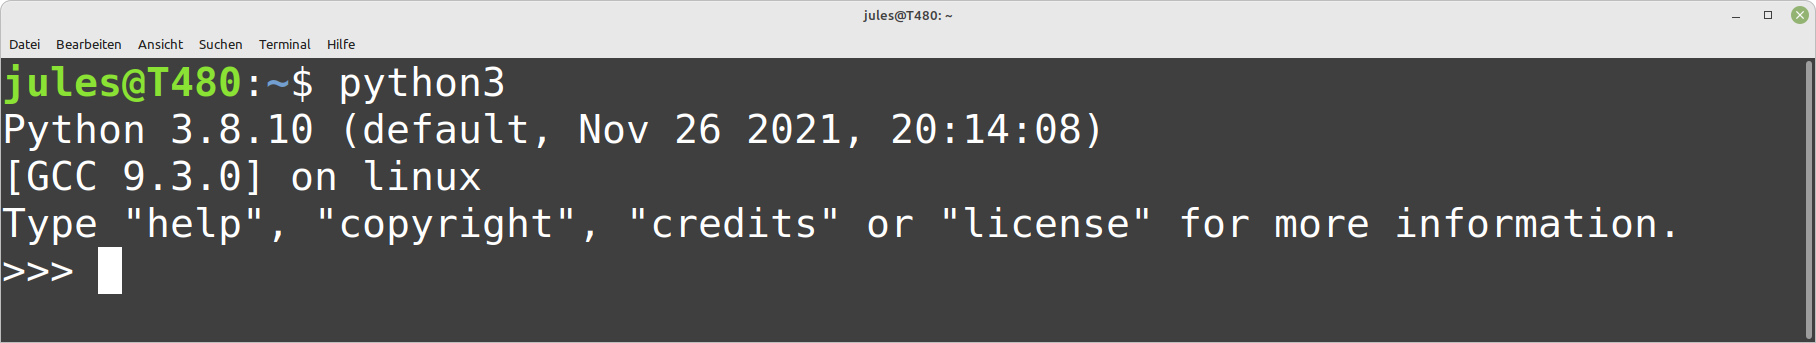
\includegraphics[width=12cm]{figures/console.png}
		\caption{Python3 REPL}
	\end{figure}
\end{frame}

\begin{frame}[fragile]
	\begin{block}{Running code}
		- REPL\\
		- python3 file args
	\end{block}
	\begin{example}
			\begin{minted}{bash}
python3 hello-world.py
		\end{minted}
	\end{example}
\end{frame}

\begin{frame}
	\frametitle{Combining Editor and Interpreter}
	\begin{figure}
		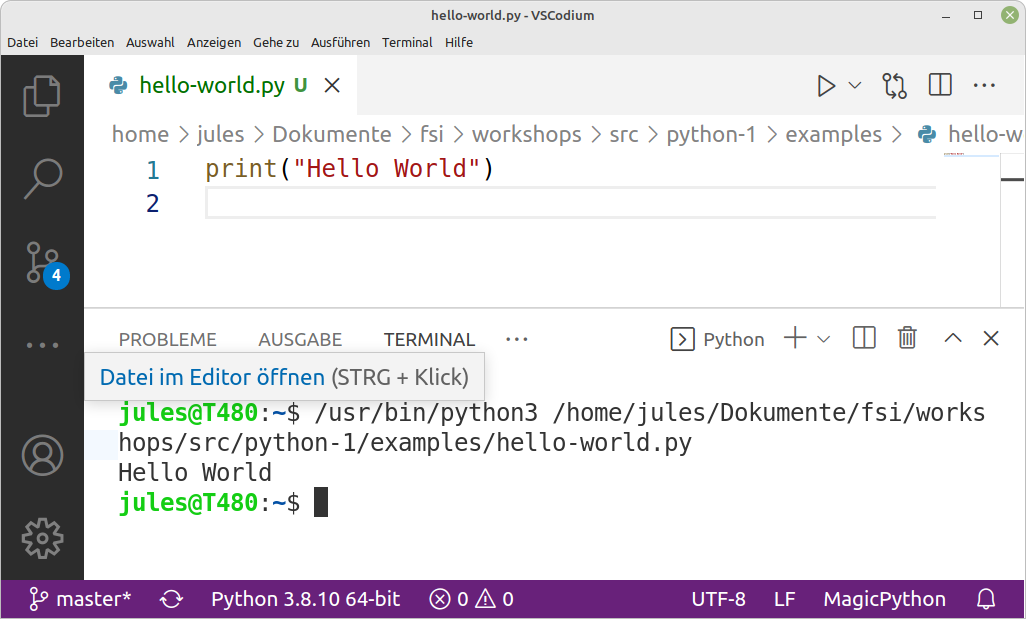
\includegraphics[width=8cm]{figures/vs-code.png}
		\caption{VS Codium}
	\end{figure}
\end{frame}
\begin{frame}
	\textbf{Possible IDEs / Editors:}\\
	- VS Codium: \url{https://vscodium.com/}\\
	- PyCharm: \url{https://www.jetbrains.com/pycharm/}\\
	- Atom: \url{https://atom.io/}\\
	- ...
\end{frame}

\begin{frame}[fragile]
	\frametitle{hello-world.py}
	- Content: \mintinline{python}{print("Hello World")}\\
	- Run it!
\end{frame}
%%%%%%%%%%%%%%%%%%%%%%%%%%%%%%%%%%%%%%%%%%%%%%%%%%%%%%%%%%%%%%%%%%%%%%%%%%%%%%%%%%%%%%%%%%%%%
% Part 2
\begin{frame}[fragile]
	\frametitle{Basic operators and types}
	Just like `any other' language.
	\begin{block}{Math}
		\begin{minted}{python}
s = (a + b - c) / d * e
p = a ** 2 # a to the power of 2
b = a^2    # bitwise shifting
m = a%2    # mod
		\end{minted}
	\end{block}
	\begin{exampleblock}{Numeric types}
	\begin{minted}{python}
int, float, complex
i = 1 = int("1") = int(1.0)
f = 4.2
c = 4+2j
	\end{minted}
\end{exampleblock}
\end{frame}
\begin{frame}[fragile]
	\begin{block}{Strings}
		\begin{minted}{python}
s = "Hello " + "World"
c = "A" * 10 + "HHHH"
S = s.upper()
length = len(S)   # Returns Integer
pos = s.find("W") # Return Integer (Position of first W)
		\end{minted}
	\end{block}
	\begin{exampleblock}{Text types}
		\begin{minted}{python}
str
s = str(1)
		\end{minted}
	\end{exampleblock}
\end{frame}

\begin{frame}[fragile]
	\begin{block}{Booleans}
		\begin{minted}{python}
a = (True or False) and not False
		\end{minted}
	\end{block}
	\begin{exampleblock}{Boolean types}
		\begin{minted}{python}
bool
t = bool(1) = bool("Not Empty")
f = bool(0) = bool("")
		\end{minted}
	\end{exampleblock}
\end{frame}

\begin{frame}[fragile]
	\begin{block}{Comparision}
		\begin{minted}{python}
<, >, ==, !=, <=, >=
		\end{minted}
	\end{block}
	\begin{example}{}
		\begin{minted}{python}
t = 3 < 5 
t = not "A" == "B"
f = 4.2 == 2
f = 0 == "Hello" # Comparision in between types is possible
		\end{minted}
	\end{example}
\end{frame}

\begin{frame}[fragile]
	\frametitle{01-types.py}
	\begin{exampleblock}{Exercise}
	Desired output: `The sum of 41.8 and 0.2 is 42'.\\
	Use following variables:
		\begin{minted}{python}
i = 41.8
f = 0.2
prefix = "The sum of "
		\end{minted}
	\end{exampleblock}
\end{frame}

%%%%%%%%%%%%%%%%%%%%%%%%%%%%%%%%%%%%%%%%%%%%%%%%%%%%%%%%%%%%%%%%%%%%%%%%%%%
% Lists / Dicts / Tuples
\begin{frame}[fragile]
	\begin{block}{Lists}<1->
Mutable, dynamic in length, non-homogenous, ordered
\begin{minted}{python}
aList = [1, 2, 3, 4, "What?", 6]
aList[0]             # -> 1
aList[4:]            # -> ['What?', 6]
aList[1::2]          # -> [2, 4, 6]  
aList[-1]            # -> 6
aList.append(7)      # -> [..., 6, 7]
aList.extend([8,9])  # -> [..., 6, 7, 8, 9]
aList[0] = "New Zero"
general form: [from:to:step/order]
\end{minted}
	\end{block}
	\begin{block}{Tuples}<2->
	Non-Mutable, fixed length, non-homogenous
	\begin{minted}{python}
aTuple = ("A", "a", 1)
a[0] 	# -> "A"
	\end{minted}
\end{block}
\end{frame}

\begin{frame}[fragile]
	
	\begin{block}{Dicts}
	Mutable, dynamic in size, non-homogenous, unordered\footnote{Somehow..}
	\begin{minted}{python}
d = {"key": "value", 1: 3}
d["key"]     # -> "value"
d["new"] = 2 # Insert new value to d
d.keys()     # -> ["key", 1, "new"]
d.values()   # -> ["value, 3, 2]
d.items()    # -> [("key", "value"), (1, 3), ("new", 2)]
	\end{minted}
	\end{block}
\textbf{See: } \url{https://docs.python.org/3/tutorial/datastructures.html}
\end{frame}
%%%%%%%%%%%%%%%%%%%%%%%%%%%%%%%%%%%%%%%%%%%%%%%%%%%%%%%%%%%%%%%%%%%%%%%%%%%%%%
% If and Loops

\begin{frame}[fragile]
	\frametitle{Control flow: if, for, while, break, continue}
	Regular control flow with if:
	\begin{minted}{python}
if condition:
  doThis()
elif cond2:
  doThat()
else:
  otherWise()
	\end{minted}
\end{frame}

\begin{frame}[fragile]
Looping has two different approaches:
\begin{block}{while / condition}<1->
	\begin{minted}{python}
i = 0
while i < 10:
  print(i)
  i = i + 1
	\end{minted}
\end{block} 
\begin{block}{for / iterable}<2->
	\begin{minted}{python}
for element in iterable:
  print(e)
	\end{minted}
\end{block} 
\end{frame}

\begin{frame}[fragile]
Iterables: something with an order and members.
\begin{example}
	\begin{minted}{python}
tuples = (0, 1,2,3,4)
lists  = [0, 1,2,3,4]
string = "Hello World"
dicts = {"a", 2}  
range(0, 6, 2) # start, stop, interval
               # somehow comparable to [0,2,4]
file objects
...
	\end{minted}
\end{example}
\end{frame}

\begin{frame}[fragile]
	\begin{block}{for / iterable}<1->
		\begin{minted}{python}
for element in iterable:
  print(e)
		\end{minted}
	\end{block}
\begin{example}<2->
		\begin{minted}{python}
for i in range(5):
  print(e) # 0, 1, 2, 3, 4
for c in "Hello World":
  print(e) # Every char
for k in {"k": "v", "k2": "v2"}:
  print(k) # Only the keys
for k, v in {"k": "v", "k2": "v2"}.items():
  print(k, v) # Unpacking
\end{minted}
\end{example}
\end{frame}

\begin{frame}[fragile]
\textbf{Unpacking}:\\
- Object with ordered members\\
- Number of vars equal to members\footnote{\mintinline{python}{x, *xs  = [1, 2, 3, 4]}  $\rightarrow$ \mintinline{python}{xs = [2,3,4]}}.
\begin{example}
	\begin{minted}{python}
a, b, c = (1, 2, 3)
a, b,   = [1,2]
	\end{minted}
\end{example}
\end{frame}

\begin{frame}[fragile]
	Exit the loop early?
	\begin{block}{Break}
	\begin{minted}{python}
while True:   # works for "for i in .." aswell 
  doThis()
  if exitCondition:
     break
	\end{minted}
	\end{block}
	Skip to the next element?
	\begin{block}{Continue}
		\begin{minted}{python}
for i in range(4):
  if i == 2:
    continue
  print(i)
-> 0, 1, 3
		\end{minted}
	\end{block}
\end{frame}


\begin{frame}[fragile]
	\frametitle{02-number-guess.py}
	\begin{exampleblock}{Exercise}
Implement a basic python number guessing game.\\
1. Generate a random number.\\
2. Ask for a guess.\\
3. Check if guess was correct.\\
4. If not, say if number was smaller / larger\\
5. Repeat from step 2, but only 8 times max.\\
~\\
Use following functions:
		\begin{minted}{python}
from random import randint
randint(0,1024)  # random integer N such that a <= N <= b
input("Number?") # Takes input from user
		\end{minted}
	\end{exampleblock}
\end{frame}


\begin{frame}[fragile]
	\frametitle{03-lists.py}
	\begin{exampleblock}{Exercise}
		Understand how to uses loops and lists.\\
E1:\\
Print the last element of list l1:
\begin{minted}{python}
l1 = ["first", "middle", "last"]
\end{minted}
E2.1:\\
Print every second element of list l2\_1\\
Without loop.
\begin{minted}{python}
l2_1 = [0,1,2,3,4,5,6,7,8,9]
\end{minted}
....
	\end{exampleblock}
\end{frame}

\begin{frame}[fragile]
	\frametitle{Deepcopy}
= creates only a reference to the object / list	
		\begin{example}
			\begin{minted}{python}
l1 = [1,2,3,4]
l2 = l1
l1.append(5)
print(l2)
[1, 2, 3, 4, 5]
			\end{minted}
		\end{example}

\begin{block}{}
\begin{minted}{python}
from copy import deepcopy
l2 = deepcopy(l1)
\end{minted}
\end{block}	
See post from `Russia Must Remove Putin': \url{https://stackoverflow.com/a/46939443/5410925}	

\end{frame}

% End of Part 2
%%%%%%%%%%%%%%%%%%%%%%%%%%%%%%%%%%%%%%%%%%%%%%%%%%%%%%%%%%%%%%%%%%%%%%%%%%%%%%%%%%%%%%%%%%%%%

% Part 3



\begin{frame}[fragile]
	\frametitle{\textbf{Part 3:} Abstraction}	
	\textbf{Functions:}\\
	- Decomposition of Code into parts\\
	- Function acts like a black bock
	\begin{minted}{python}
def is_even(i):
  """
  Computes if an integer is even.
  Input:
  	i: int
  Returns:
  	even: bool, result.
  """
  even = (1 % 2) == 0
  return even
\end{minted}
\end{frame}

\begin{frame}[fragile]
	\frametitle{\textbf{Part 3:} Abstraction}	
	\textbf{Functions:}\\
	- Decomposition of Code into parts.\\
	- Function acts like a black bock.
	\begin{minted}{python}
def is_even(i):          <- keyword, name(parameters)
  """                    _
  Is integer is even?     |
  Input:                  |
    i: int                |> DocString
  Returns:                |
    even: bool, result.   |
  """                    _|
  even = (1 % 2) == 0     <- Computation
  return even             <- Return (Optional)
	\end{minted}
\end{frame}


\begin{frame}[fragile]
	\begin{example}
\begin{minted}{python}
def noReturn(a, b):
  print(a)

def optionalArgument(a, b=0):
  return

def optionalReturn(x):
  if x < 5:
    return True
 
def polymorphicReturn(x):
  if x < 5:
    return True
  return x
\end{minted}
	\end{example}
\end{frame}


\begin{frame}[fragile]
	\textbf{Modules / Import:}\\
	- Full:~~~~~\mintinline{python}{import moduleName}\\
	- Partial: \mintinline{python}{from moduleName import subModule} \\
	- File in same directory: \mintinline{python}{import filename}\\
	- A lot of standard libraries:
	\begin{itemize}
		\item Math: random, statistics, math
		\item Time: time, datetime 
		\item OS/IO: argparse, os, pathlib, sys
		\item Network: urllib3
	\end{itemize}
	- See: \url{https://docs.python.org/3/library/index.html}\\
	- Extended standard: numpy, pandas, ...
	
	
\end{frame}

\begin{frame}[fragile]
	\textbf{Scope:}\\
	- Which variables are visible from which part of the code.\\
	- From outer to inner.\\
	\begin{example}
		\begin{minted}{python}
def useX(y):
  return y + x

def modifyX(y):  
  x = y + x

x = 10
y = useX(5)
modifyX(y)
print(x)
		\end{minted}
	\end{example}
\end{frame}

\begin{frame}[fragile]
	\textbf{Scope:}\\
	- Which variables are visible from which part of the code.\\
	- From outer to inner.\\
	\begin{example}
		\begin{minted}{python}
def useX(y):
  return y + x
		
def modifyX(y):  
  x = y + x <- Assignment forces x to be local variable
            -> Error: local variable 'x'
	       referenced before assignment
x = 10
y = useX(5)
modifyX(y)
print(x)
		\end{minted}
	\end{example}
\end{frame}

\begin{frame}[fragile]
	\frametitle{scope.py}
	\begin{example}
		\begin{minted}{python}
def g(x):
  def h():
	x = 'abc'
  x = x + 1
  print(f"x in g: {x}")
  h()
  return x
		
x = 3
print(f"x at position 2: {x}")
z = g(x)
print(f"z at position 1: {z}")
		\end{minted}
	\end{example}
\end{frame}

\begin{frame}[fragile]
	\textbf{lambda functions}:\\
	- good for single use functions\\
	- usually defined inline\\
	- useful for currying
\begin{example}{}
\begin{minted}{python}
l = [0,1,2,3,4,5,6,7,8,9]
lPow = map(lambda x: pow(x,2), l)

equiv to: [pow(x,2) for x in l]	

\end{minted}
\end{example}
\end{frame}

\begin{frame}[fragile]
	\textbf{File reading}:\\
	- Files need to be opened and closed.\\
	- We don't want to handle that...\\
	\begin{example}
		\begin{minted}{python}
with open("path/file.txt", "r") as f:
  line = f.readline()
  content = f.read() # reads everything

with open("path/file.txt", "r") as f: 
  for line in f:
    print(line)
		\end{minted}
		Modes:\\
		- r, read\\
	\end{example}
\end{frame}
\begin{frame}[fragile]
	\textbf{File writing}:\\
	\begin{example}
		\begin{minted}{python}
with open("path/file.txt", "w") as f:
  f.write("string")
  f.write("\n")
  f.writelines(["line1", "l2", "l3"])
	\end{minted}
		Modes:\\
		- w, overwrite / write\\
		- a, append\\
		- x, write, error if file exist
	\end{example}
\end{frame}

\begin{frame}[fragile]
	\frametitle{06-wordle.py}
	\begin{figure}
		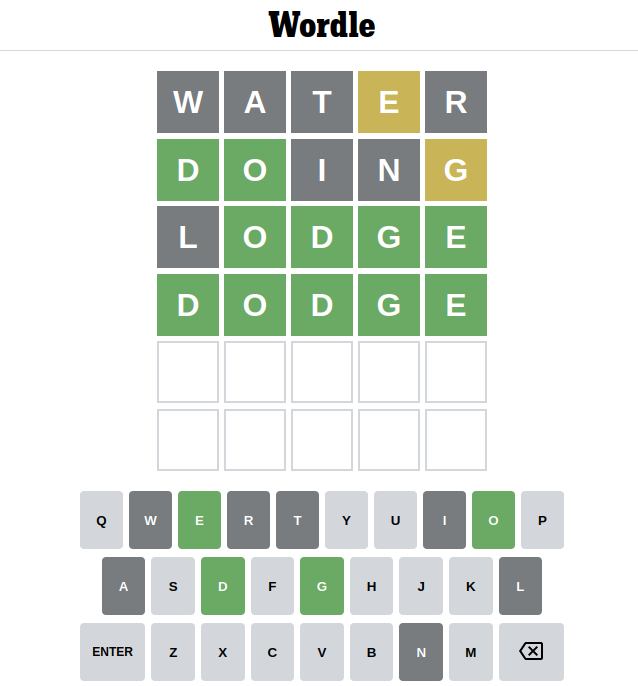
\includegraphics[width=6cm]{figures/wordle.png}
		\caption{Wordle by NYTimes, \url{https://www.nytimes.com/games/wordle}}
	\end{figure}
\end{frame}

\begin{frame}[fragile]
	\frametitle{06-wordle.py}
	\begin{figure}
		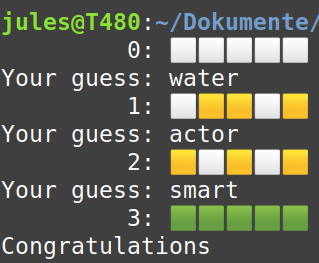
\includegraphics[width=5cm]{figures/wordle_terminal.png}
		\caption{Our goal.}
	\end{figure}
\end{frame}

\begin{frame}[fragile]
	\frametitle{Objects / Class}
	- Object is instance of an Class.\\
	- Has properties and methods. \\
	- Everything is a object.\\
\begin{block}{Class}
	
	\begin{minted}{python}
class MinimalClass():
  def __init__(self):
    pass
	\end{minted}
\end{block}	
\begin{block}{Object}
\begin{minted}{python}
x = MinimalClass()
\end{minted}	
\end{block}	
\end{frame}

\begin{frame}[fragile]
\textbf{Functions defined in a class}:\\
- are applied on an object.\\
- requires at least one argument (self).

\begin{example}
 \begin{minted}{python}
class Counter():
  def __init__(self, x):
    self.x = x

  def addOne(self):
    self.x = self.x + 1
    
c = Counter(0)
c.addOne()
print(c.x)
\end{minted}	
\end{example}
\end{frame}


\begin{frame}[fragile]
	\textbf{Functions defined in a class}:\\
	- are applied on an object.\\
	- requires at least one argument (self).
	
	\begin{example}
		\begin{minted}{python}
class Counter():
  def __init__(self, x):
    self.x = x       <- property
	
  def addOne(self):  <- self required
	self.x = self.x + 1
		
c = Counter(0)       <- calling __init__
c.addOne()           <- alling addOne()
print(c.x)           <- accessing property
		\end{minted}	
	\end{example}
\end{frame}


\begin{frame}[fragile]
	\textbf{Style / Information hiding}:\\
	- Use getter / setter method outside of class\\
	- Information hiding is NOT possible\\\\
	\textbf{Inheritance}:
	\begin{example}
		\begin{minted}{python}
class Animal():
  def __init__(self, name):
    self.name = name
    
class Cat(Animal):
  def speak(self):
	print("Meow")

Cat("Kleopatra").speak()
		\end{minted}
	\end{example}
\end{frame}

\begin{frame}[fragile]
	\textbf{Magic Methods}\footnote{A complete guide: \url{https://rszalski.github.io/magicmethods/}}:\\
	- Adds `magic' to a class.\\
	- Start / end with \mintinline{python}{__} . Example: \mintinline{python}{__init__}\\
	- Comparison, Type Conversion, Representation, Context
	
	\begin{example}
		\begin{minted}{python}
Cat("Kleopatra") == Cat("Kleopatra") 
--> False (two different objects)
		\end{minted}
	\end{example}
\end{frame}

\begin{frame}[fragile]
	\textbf{Magic Methods}\footnote{A complete guide: \url{https://rszalski.github.io/magicmethods/}}:\\
	- Adds `magic' to a class.\\
	- Start / end with \mintinline{python}{__} . Example: \mintinline{python}{__init__}\\
	- Comparison, Type Conversion, Representation, Context
	
	\begin{example}
		\begin{minted}{python}
Cat("Kleopatra") == Cat("Kleopatra") 
--> False (two different objects)

class Animal():
  def __eq__(self, other):
  	return self.name == other.name
  
--> Cat("Kleopatra") == Cat("Kleopatra") -> True
		\end{minted}
	\end{example}
\end{frame}

\begin{frame}[fragile]
	\begin{exampleblock}{Comparision}
		\begin{tabular}{ll}
Equality:&\mintinline{python}{__eq__(self, other)}\\
Greater than:~~&\mintinline{python}{__gt__(self, other)}\\
Less than: &\mintinline{python}{__lt__(self, other)}\\
... &
		\end{tabular}
	\end{exampleblock}
\begin{exampleblock}{Arithmetic}
			\begin{tabular}{ll}
Addition:&\mintinline{python}{__add__(self, other)}\\
Multiplication:& \mintinline{python}{__mul__(self, other)}\\
...&
\end{tabular}
\end{exampleblock}	
\begin{exampleblock}{Sequences}
			\begin{tabular}{ll}
Iterator:~~~~~~~~~&\mintinline{python}{__iter__(self)}\\
Reversed:&\mintinline{python}{__reversed__(self)}\\
... &
\end{tabular}
\end{exampleblock}
\end{frame}

\begin{frame}[fragile]
	\frametitle{07-objects.py}
\begin{exampleblock}{Exercise}
\textbf{Goal}: Implement a Vector-Class with following properties:\\
~\\
1: Holds values for x, y, z\\
~~~ Example: V1 = Vector(1,2,3)\\
2: Equal \mintinline{python}{__eq__}\\
3: Print \mintinline{python}{__str__}\\	
4: Vectors can be added, this will return a new vector\\
~~~ Example: \mintinline{python}{V1 + V1 -> Vector(2,4,6)}\\
5: Extend code so that \mintinline{python}{V1.add(Vector(2,3,4))} will mutate V1.\\
~~~ We do not want to see duplicated code.\\
~~~ Remember: use \mintinline{python}{deepcopy} to clone an object.
\end{exampleblock}
	
\end{frame}

\begin{frame}[fragile]
	\frametitle{Exceptions}
	- Error will raise an exception.\\
	~~$\rightarrow$ terminates programme.\\
	- We can catch and raise them.
	\begin{block}{Raise}
		\begin{minted}{python}
raise Exception("Your error message")
		\end{minted}
	\end{block}
	\begin{block}{Catch}
\begin{minted}{python}
try:
  y = 1 / x
except:
  y = float("-inf")
else:    <- optional
  print("everything ok")
\end{minted}	
	\end{block}
\end{frame}

\begin{frame}[fragile]
	\textbf{Exception types}\footnote{Complete list: \url{https://docs.python.org/3/library/exceptions.html}}:\\
	Be more specific while raising / catching exceptions! 
	\begin{exampleblock}{Types}
	- ZeroDivisionError\\
	- IndexError (lists)\\
	- KeyError (dicts)\\
	- TypeError (wrong type, forgot to cast?)
	\end{exampleblock}
	\begin{example}
\begin{minted}{python}
try:
  y = 1 / x
except ZeroDivisionError:
  y = float("-inf")
except Exception as e:
  print("Other error:" , e)
\end{minted}
	\end{example}

\end{frame}

\begin{frame}[fragile]
\centering
\LARGE
Thank You!
	
\end{frame}

\end{document} 